\documentclass[10pt,a4paper]{book}
\usepackage[latin1]{inputenc}
\usepackage{amsmath}
\usepackage{amsfonts}
\usepackage{amssymb}
\usepackage{graphicx}
\author{Daniel Frederico Lins Leite}
\title{Asymptotic Statistics}
\begin{document}
\maketitle
\tableofcontents

\chapter {Introduction}

The idea of this crash course on asymptotic Statistics is to have all proofs and ideas related with the one of the three most important aspects of statistics, being estimation. The other two being confidence interval and hypothesis testing, off course.\\

The idea is to present as gentle as possible the needed concepts to follow a more thorough course. Here one will find the concepts of "asymptotic", "estimators", Markov and Chebyshevs inequalities, convergnce in the sense for Statistics, characteristic functions, the weak law of large numbers and the Central Limit Theorem.
	
\chapter{Asymptotic Behaviour of Estimators}
\section{Introduction}

As "Asymptotic Statistics" we understand the study of Probabilities and Statistics as one of its parameters go to infinity. We will study for example:

\begin{align}
	\lim_{n->\infty}{P(X_n \in A)}
\end{align}

or 

\begin{align}
	\lim_{n->\infty}{P((X_n - X) \in A)}
\end{align}

Here $P(x \in A) = \int_{A}{f(x)dx}$. The lower-case $f$ has a especial meaning because that is how we label the PDF of a distribution. We use upper-case $F$ to mean de CDF. We also know that to be a valid "random variable":

\begin{align}
	\int_{-\infty}^{\infty}{f(x)dx} = 1 && f(x) >= 0
\end{align}

Where $X_n$ means off course a "random variable", pure in the sense that is obeys a known distribution or a "transformed random variable". We will be interested to know if a "random variable" converge to a constant, to another "random variable" of if it diverge. Throughout this book we will see that we can conclude different things if any of these cases are proved as true.

One of the most interesting, or one the most useful, "random variables" is the "estimator". We call "estimator" any "statistic" that does not depend on any of the "population parameters" an possible estimator. If on top of that we define that this "statistic" will be used as an "estimation" of the "population parameter", we have a "estimator".

A famous statistic is the "sample mean" that we will define as:

\begin{align*}
	X_i \sim P_{\theta}\\
	S_n = \sum_{\forall i}{X_i}\\
	\bar{X_{n}} = \frac{S_n}{n}\\
\end{align*}

We understand the expressions above as:
\begin{itemize}
	\item {$X_i$ is a "random variable" that follows a distribution described with a parameter $\theta$, that can be a number or various numbers;}
	\item {The set of all $X_i$ are i.i.d.}
	\item {$S_n$ is another "random variable". Being the sum of $n$ "random variables" allows us to know the distribution of $S_n$ in some cases}
	\item {$\bar{X_{n}}$ is another "random variable" that applies the "transformation" $1/x$ to the "random variable" $S_n$}
\end{itemize}

Being random variables, $X_i$, $S_n$, $\bar{X_{n}}$, allow them to have "expected values", "variations" and any other statistics themselves. This is a powerfull source of confusion. So we can have:

\begin{align*}
	E[X_i] = a \text{ or } f_a(i)\\	
	E[S_n] = b \text{ or } f_b(n)\\
	E[\bar{X_{n}}] = c \text{ or } f_c(n)\\
\end{align*}

In these cases, $a$, $b$, $c$ are not "random variables". They are constants, or functions that depend on the "random variables" "parameter". The same can be said about their "variance" and other statistics.

Remember that "Expected Value" is:

\begin{align}
	E[X] = \int_{-\infty}^{\infty}{x*f(x)dx}
\end{align}

Actually this is just the "First Moment" of $X$. We can the n-th "moment" as:

\begin{align}
	\int_{-\infty}^{\infty}{x^n*f(x)dx}
\end{align}

or

\begin{align*}
	E[X^1] = \int_{-\infty}^{\infty}{x^1*f(x)dx}\\
	E[X^2] = \int_{-\infty}^{\infty}{x^2*f(x)dx}\\
	...\\
	E[X^n] = \int_{-\infty}^{\infty}{x^n*f(x)dx}\\
\end{align*}

And this allows us to calculate the variance as, the "second moment" minus the square of the "first moment":

\begin{align}
	\text{VAR}[X] = E[X^2] - E[X]^2
\end{align}

\section{Markov's Inequality Intuition}
	
What can you say about a "Probbility distribution" if you only have its mean? Probably not much. But not much is more than nothing. If we imagine a standard dice with six faces, but not necessarily fair, each face having the same probability. The question is, knoning just the mean, can we affirm with a 100\% certainity that the dice is not fair?

For example, if someone tell us that the $E[X_i]$, $X_i$ being a roll of the dice is $6$. We know that the only way of this happening is when $P(X = 6) = 1$ and $P(X < 6) = 0$ because of the "Expected Value" definition.

\begin{align*}
	E[X] &= \sum_{i=1}^{6}{i*P(X=i)} = 6\\
	&= 6*P(X=6) = 6\\
	& P(X=6) = \frac{6}{6}\\
	& P(X=6) = 1\\
\end{align*}

So it seems that knowing only the $E[X]$ allows us to take some conclusions of the distribution. But this is a extreme case. Can we take conclusions if for example the $E[X]$ is the same as the "expected value" when the dice is fair? Let us see.

We know that the $E[X]$ is:

\begin{align*}
	E[X] &= \sum_{i=1}^{6}{i*P(X=i)}\\
\end{align*}

And we know that $i \in {1,2,3,4,5,6}$ or $i > 0$. We know that $i$ is positive. We also know that $P(X = i) \in [0,1]$. It is also positive. The multiplication of two positive values is also positive. And the sum of two positive values is also positive.

\begin{align*}
	i &> 0\\
	P(X = i) &> 0\\
	a * b &> 0 \text{, if } a > 0 \text{ and } b > 0\\
	a + b &> 0 \text{, if } a > 0 \text{ and } b > 0	
\end{align*}

Which give us that 

\begin{align*}
	E[X] &= \sum_{i=1}^{6}{i*P(X=i)}\\
	&= \sum_{i=1}^{5}{i*P(X=i)} + 6*P(X=6)
\end{align*}

We know that this summuation is going to be greater than zero. Whick make the $E[X]$ greater than or equal $6*P(X=6)$. In the extreme case above, it was equal because the summation was zero. But the summation can be greater than zero (never lower).

\begin{align*}
	E[X] &= \sum_{i=1}^{6}{i*P(X=i)}\\
	E[X] &= \sum_{i=1}^{5}{i*P(X=i)} + 6*P(X=6)\\
	E[X] &>= 6*P(X=6)\\
	\frac{E[X]}{6} &>= P(X=6)\\
	P(X=6) &<= \frac{E[X]}{6}
\end{align*}

Which is quite surprising if you think. But looking from another perspective, it is quite obvious that there is a relationship with the $P(X=6)$ and the "expected value".
	
\section{Markov's Inequality}

This relationship was discovered by two mathematicians:\\	
Andrey Markov\\
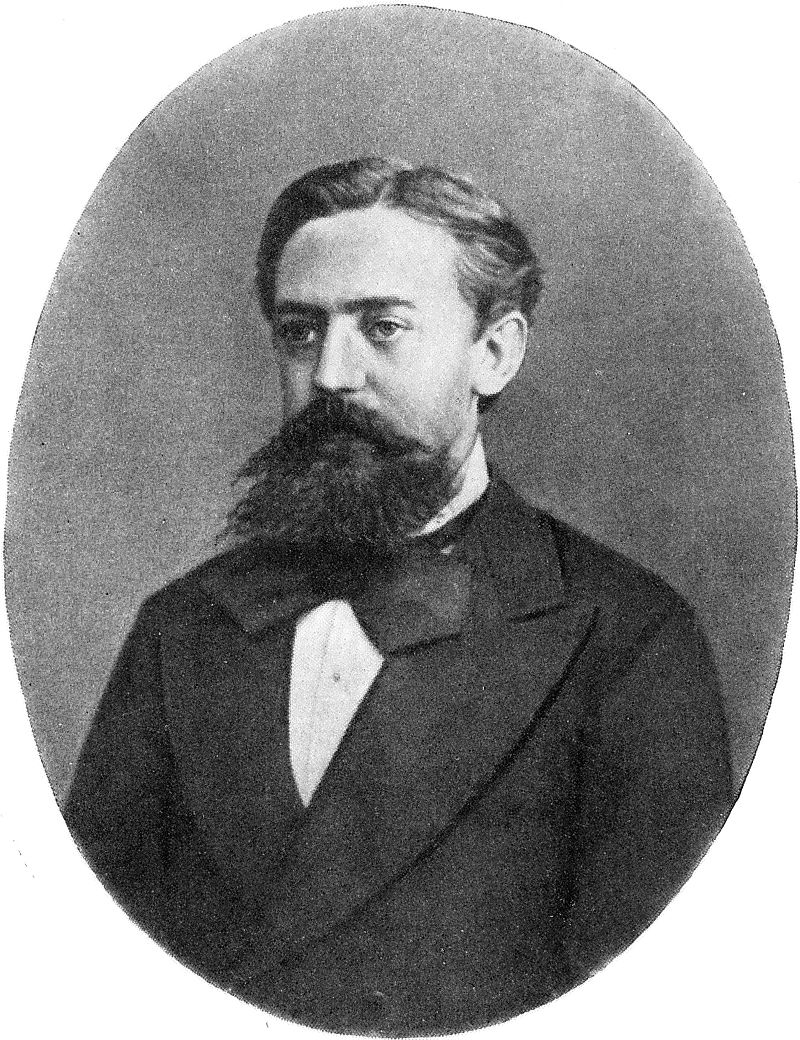
\includegraphics[width=50px]{AAMarkov}\\

and Pafnuty Chebyshev\\
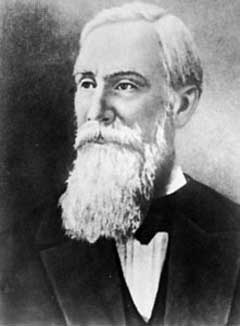
\includegraphics[width=50px]{Chebyshev}\\

And it is generalized as:
\begin{itemize}
	\item {$X$ is a nonnegative random variable;}
	\item {$a > 0$}
\end{itemize}	

We now that:

\begin{align*}
	E[X] &= \int_{-\infty}^{\infty}{x*f(x)dx}\\
	&= \int_{0}^{\infty}{x*f(x)dx} && \text{because of } X > 0\\
	&= \int_{0}^{a}{x*f(x)dx} + \int_{a}^{\infty}{x*f(x)dx} && \text{because of } a > 0\\	
\end{align*}

We know that $\int_{0}^{a}{x*f(x)dx} > 0$, so

\begin{align*}
	E[X] &= \int_{0}^{a}{x*f(x)dx} + \int_{a}^{\infty}{x*f(x)dx}\\
	E[X] &= b + \int_{a}^{\infty}{x*f(x)dx} && b > 0\\
	E[X] - b &= \int_{a}^{\infty}{x*f(x)dx}\\
	E[X] &>= \int_{a}^{\infty}{x*f(x)dx} && b > 0\\
\end{align*}

Before the next step, we must realize that:

\begin{align*}
	\int_{a}^{\infty}{x*f(x)dx}&\\
	&=\int_{a}^{\infty}{(a+(x-a))*f(x)dx}\\
	&=\int_{a}^{\infty}{a*f(x)dx}+\int_{a}^{\infty}{(x-a)*f(x)dx}\\
\end{align*}

We must realize the in the second integration, $x>=a$ and $f(x) > 0$ which makes the second integration greater than or equal to zero. This allow us to:

\begin{align*}
	\int_{a}^{\infty}{x*f(x)dx} &=\int_{a}^{\infty}{a*f(x)dx}+\int_{a}^{\infty}{(x-a)*f(x)dx}\\
	\int_{a}^{\infty}{x*f(x)dx}	&=\int_{a}^{\infty}{a*f(x)dx}+c\\
	\int_{a}^{\infty}{x*f(x)dx}	- c &=\int_{a}^{\infty}{a*f(x)dx}\\
	\int_{a}^{\infty}{x*f(x)dx}	&>= \int_{a}^{\infty}{a*f(x)dx}\\	
\end{align*}

We can use this fact with the fact that if $a>b$ and $b>c$ then $a>c$, and finish our proof

\begin{align*}
	E[X] &>= \int_{a}^{\infty}{x*f(x)dx} && b > 0\\
	E[X] &>= \int_{a}^{\infty}{a*f(x)dx} && \text{see above}\\
	E[X] &>= a*\int_{a}^{\infty}{f(x)dx}\\
	E[X] &>= a*P(X>a)\\
	\frac{E[X]}{a} &>= P(X>a)\\
\end{align*}
\begin{align}
	P(X>a) &<= \frac{E[X]}{a}	
\end{align}

Which is the obivious generalization we did in the intuition section. But remember that we are studying "Asymptotic Statistics", this is useful for us, because in some cases, the right side will depend on $n$, and in the limit the right side will converge or diverge. This will give even more information about the "random variable". All of this with just its "expected value".
		
	\section{Chebyshev's Inequality}

	\chapter{Convergence}
	\section{Convergence in probability of a random variable}
	\section{Convergence in probability to a random variable}
	\section{Convergence in probability of a random variable to a constant}
	\section{Convergence in distribution of a random variable}
	
	\chapter{Characteristic Functions}
	\section{Introduction}

	\chapter{Weak Law of Large Numbers}
	\section{Introduction}
	\section{Proof of the weak law of large numbers}
	\section{Proof using characteristic functions}
	
	\chapter{Central Limit Theorems}
	\section{Introduction}
	\section{Proof}
	\section{The Characteristic Function of a Normal Random Variable}
\end{document}